\documentclass[12pt]{iopart}

\usepackage[margin=2.5cm]{geometry}
%\usepackage{natbib} %aas uses natbib
\usepackage{setstack}
\usepackage{amsmath}
% paragraph spacing
\setlength{\parskip}{.7em}
\setlength{\parindent}{0em}

% maths/symbols

\usepackage{amssymb}

% figures
\usepackage{graphicx}
\graphicspath{{./figures/}}
\usepackage{subcaption} % subfigures

% positioning of figures and tables
\usepackage{float}

% hyperlinks
\usepackage{hyperref}


\date{October 2023}




\begin{document}
\title{Mid-Infrared Analysis of Accreting Supermassive Black Holes}
\author{Mitchell Hooymans $^1$, Michael Cowley (Supervisor) $^1$}
\address{$^1$ Queensland University of Technology, Brisbane, Australia, 4000}

\begin{abstract}
    Abstract of this Project
\end{abstract}

\ioptwocol
\section{Introduction}
Accreting Supermassive Black Holes, also called Active Galactic Nuclei (AGN), are incredibly compact and energetic regions of space that exist in the centre of some galaxies. These AGN are thought to play a role in the evolution of their host galaxies with the effect of AGN on star formation rate being an ongoing field of research \cite{cowley_zfourge_2016}. These supermassive objects are surrounded by diffuse material that spirals toward the central black hole, the transfer of angular momentum by the material causes it to heat up forming an ultra-hot accretion disc \cite{shakura_black_1973}. Outside of this accretion disc lies a doughnut-like structure of gas and dust, known as the dusty torus. This dusty torus extends from a few parsecs to a hundred parsecs from the central area of the AGN \cite{netzer_revisiting_2015}. Dust from the dusty torus can obscure AGN preventing these objects from being observed. Fortunately, emissions from the galactic nuclei are absorbed by the surrounding dusty torus and re-emit in the mid-infrared (MIR) which has a distinctive spectral energy distribution (SED)\cite{lyu_polar_2018}. Due to the infrared (IR) colours that are produced by AGN in this way, it is often possible to separate AGN observations from those of luminous star-forming galaxies \cite{hickox_obscured_2018}.
Due to this distinctive energy distribution we can observe these galaxies in specific IR colour bands, and create criteria to select AGN candidates using the fluxes in these colour bands \cite{lacy_obscured_2004, stern_midinfrared_2005, donley_identifying_2012, messias_new_2012}. These techniques work by using technique-specific empirical selection criteria to make selections of AGN candidates on colour-colour diagrams. In a colour-colour diagram the colour is the difference in magnitude for a source in two different passbands \cite{bessell_ubvri_1990}. In addition to IR selection techniques, x-ray selection techniques are thought to be a robust method for selecting AGN with x-ray AGN signatures often being present in AGN identified with other wavelength techniques such as IR, optical or radio \cite{brandt_cosmic_2015}. In this paper, we attempt to select AGN from the Fourstar Galaxy Evolution Survey (ZFOURGE) \cite{straatman_fourstar_2016} using IR and x-ray techniques. Additionally, we attempt to quantify the reliability and completeness of these metrics against a sample of true AGN. To facilitate the x-ray selections we cross-match data from the Chandra Deep Field South 4Ms Source Catalogue \cite{xue_chandra_2011} to determine x-ray data for sources present in ZFOURGE. This paper assumes a $\Lambda CDM$ model with $H_0 = 70 km \ s^{-1} \ Mpc^{-1}$, $\Omega_M = 0.3$, and $\Omega_{\Lambda} = 0.7$ 
\section{Astronomical Data}
\subsection{ZFOURGE and Supplementary Data}
For this project, the data we used was from the ZFOURGE Survey \cite{straatman_fourstar_2016}. This survey observed over 60000 galaxies in three legacy fields, CDFS \cite{giacconi_chandra_2002}, COSMOS \cite{scoville_cosmic_2007}, and UDS \cite{lawrence_ukirt_2007} each pointing covering $11' \times 11'$. Observations in ZFOURGE were made using the FourStar Infrared Camera mounted on the Magellan Baade Telescope in Las Campanas, Chile \cite{persson_fourstar_2013}. Using the FourStar instrument, ZFOURGE observes with five near-infrared (NIR) medium band filters; $J_1$, $J_2$, $J_3$, $H_s$, $H_l$ and one broad band filter $K_s$. In addition to this, the ZFOURGE survey is supplemented with multi-wavelength data from CANDELS \cite{grogin_candels_2011, koekemoer_candels_2011} and data from the Spitzer Space Telescope's IRAC \cite{fazio_infrared_2004} and MIPS \cite{rieke_multiband_2004} instruments. Additional information regarding the ZFOURGE survey, including a complete list of auxiliary data and processing, can be found in Straatman's ZFOURGE paper \cite{straatman_fourstar_2016}.
\subsection{Crossmatching}
X-ray data was crossmatched from the Chandra Deep Field-South 4Ms Survey \cite{xue_chandra_2011} with ZFOURGE data in the CDFS field to allow the selection of AGN that produce x-ray emissions \cite{szokoly_chandra_2004}. To accomplish this both catalogues were imported and crossmatching was accomplished by matching celestial coordinates using the Astropy package \cite{the_astropy_collaboration_astropy_2013}. To ensure that the cross-match is well constrained a maximum separation error of one-arcsecond radius is used. The cross-match successfully matches the celestial coordinates between each survey with each source having an almost identical right ascension and declination (See Figure 1).
\begin{figure}[h]
  \centering
  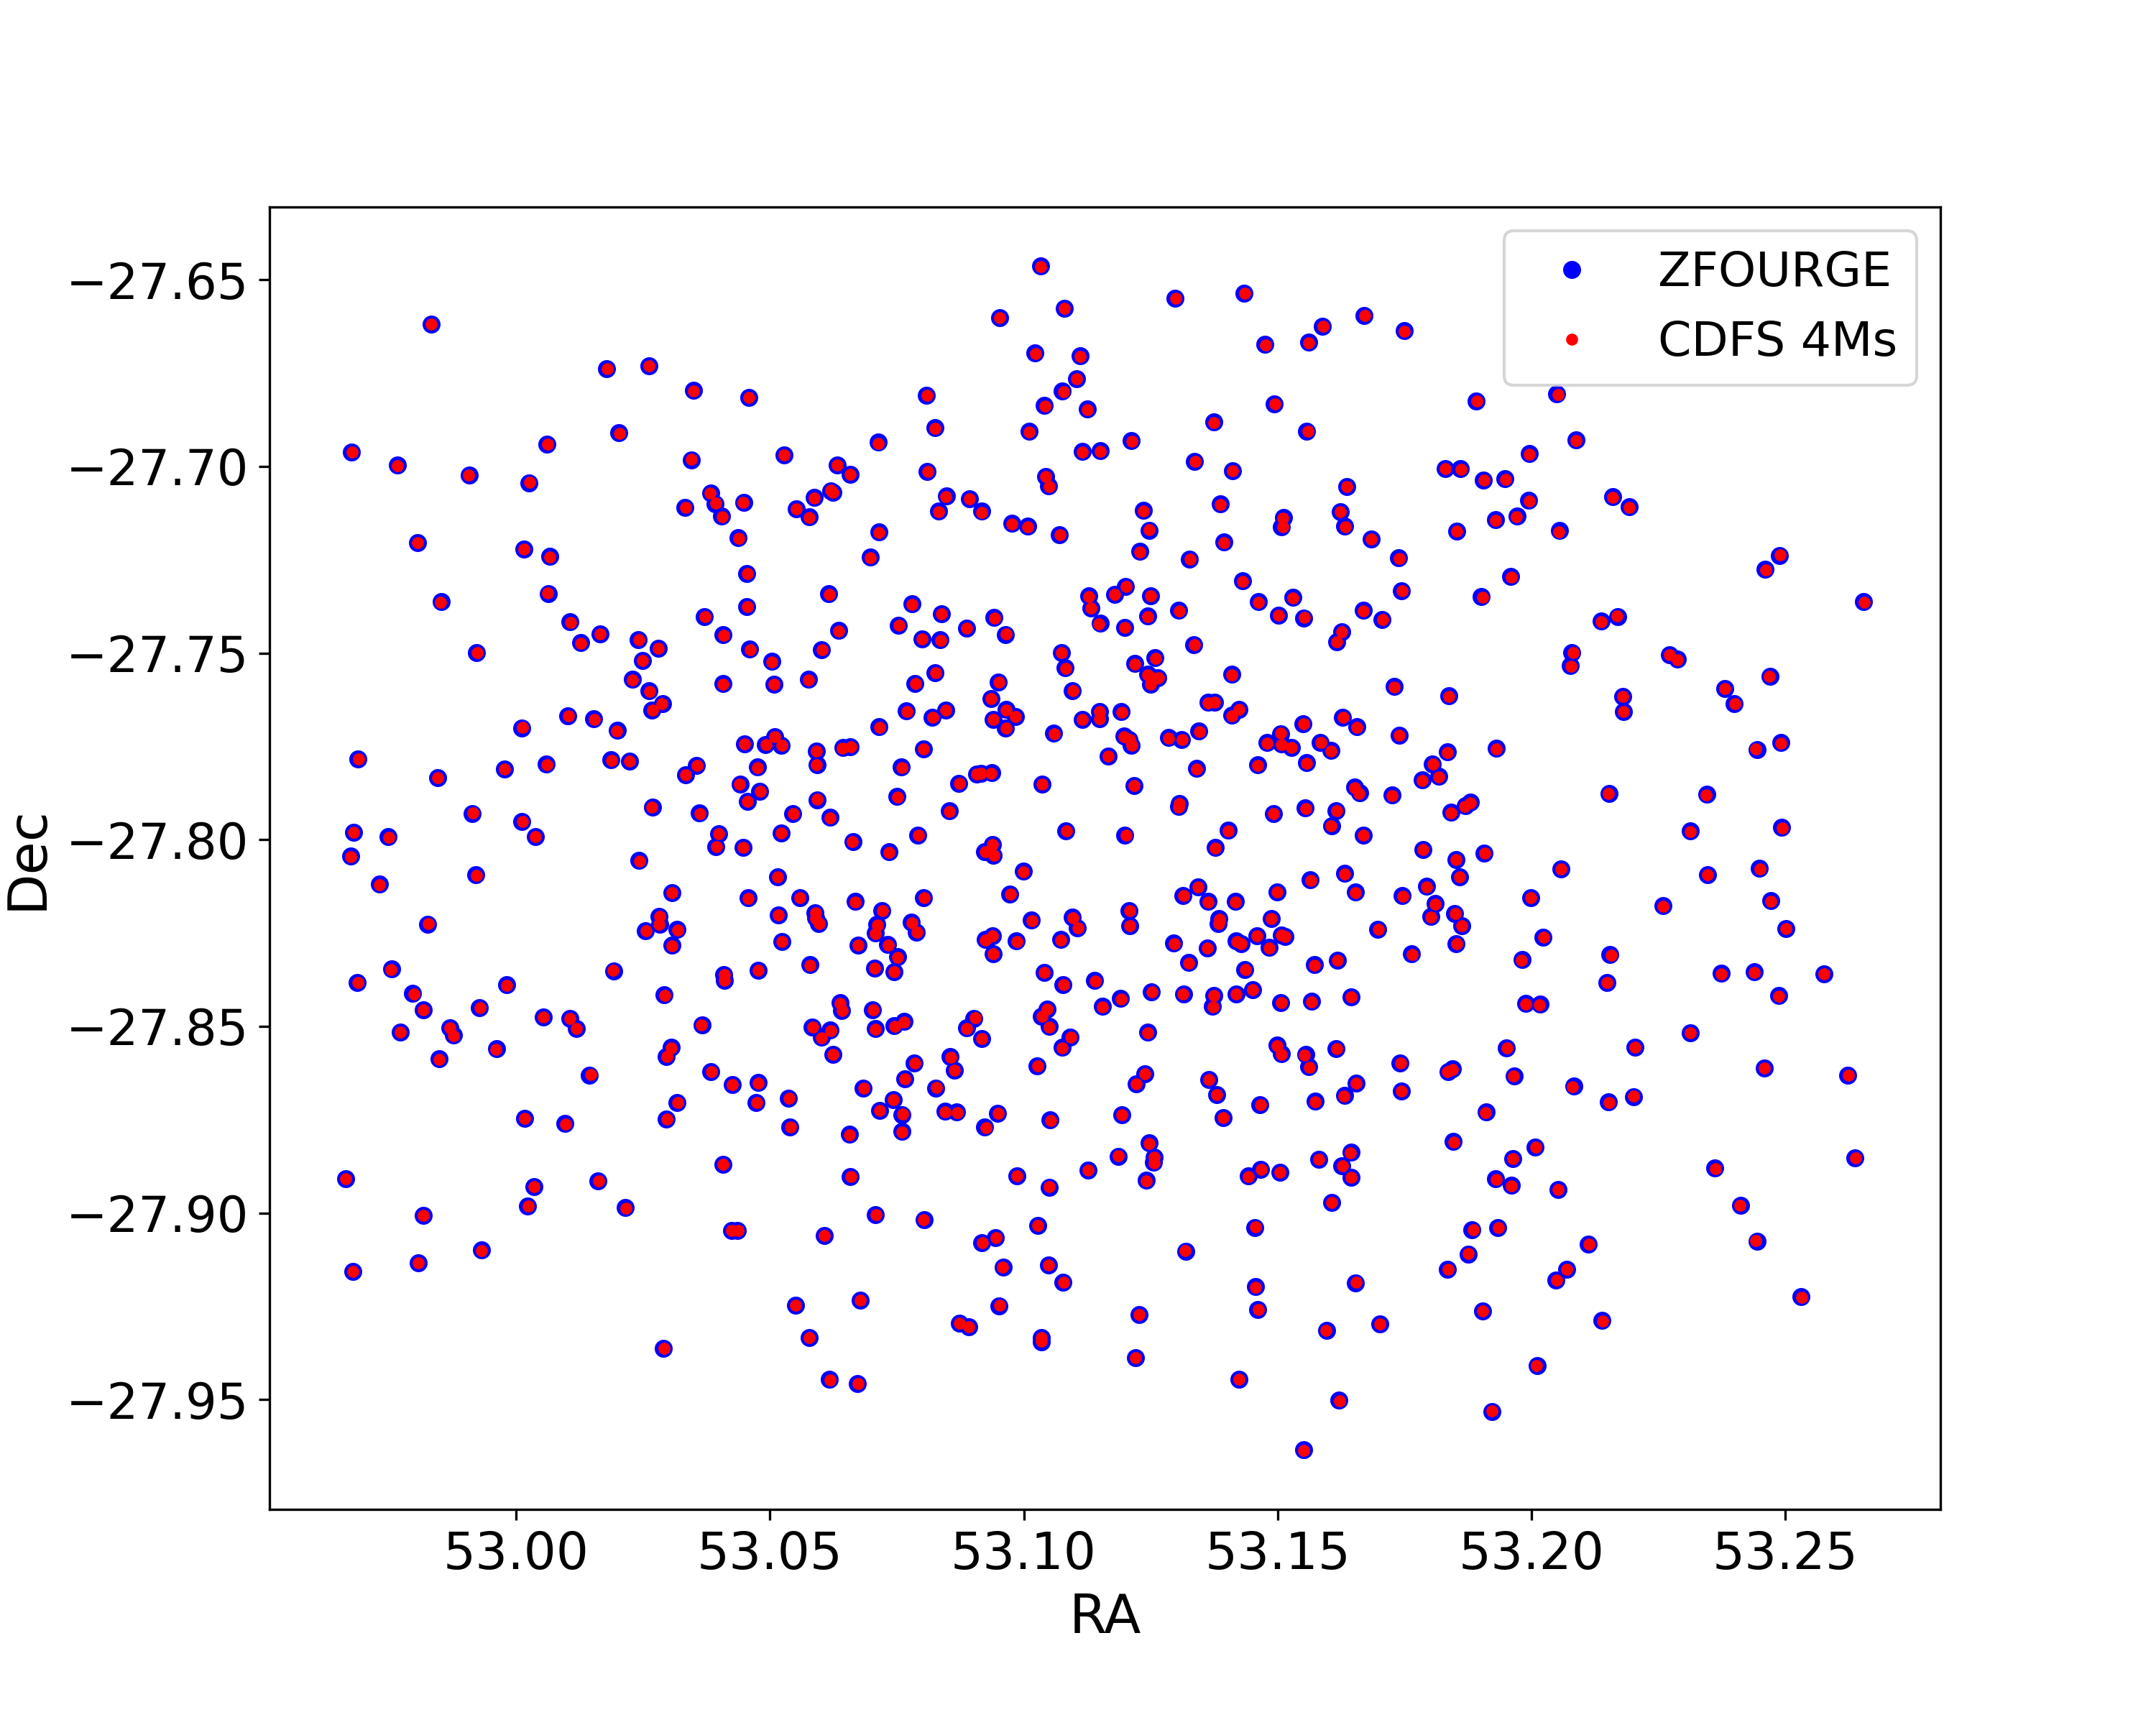
\includegraphics[width=0.49\textwidth]{plots/CDFS_4Ms_Xray_ZFOURGE_XMatch.png}
  \caption{Celestial Coordinate cross-matching between the ZFOURGE Survey in the CDFS field and the CDFS 4Ms survey.}
  \label{fig:Crossmatch}
\end{figure}
To confirm the accuracy of the cross-match, and to ensure that sources had a low likelihood of being mismatched, a distribution of the separations between sources was generated (See Figure 2). Ultimately from this cross-match 593 sources were cross-matched between both surveys. 
\begin{figure}[h]
  \centering
  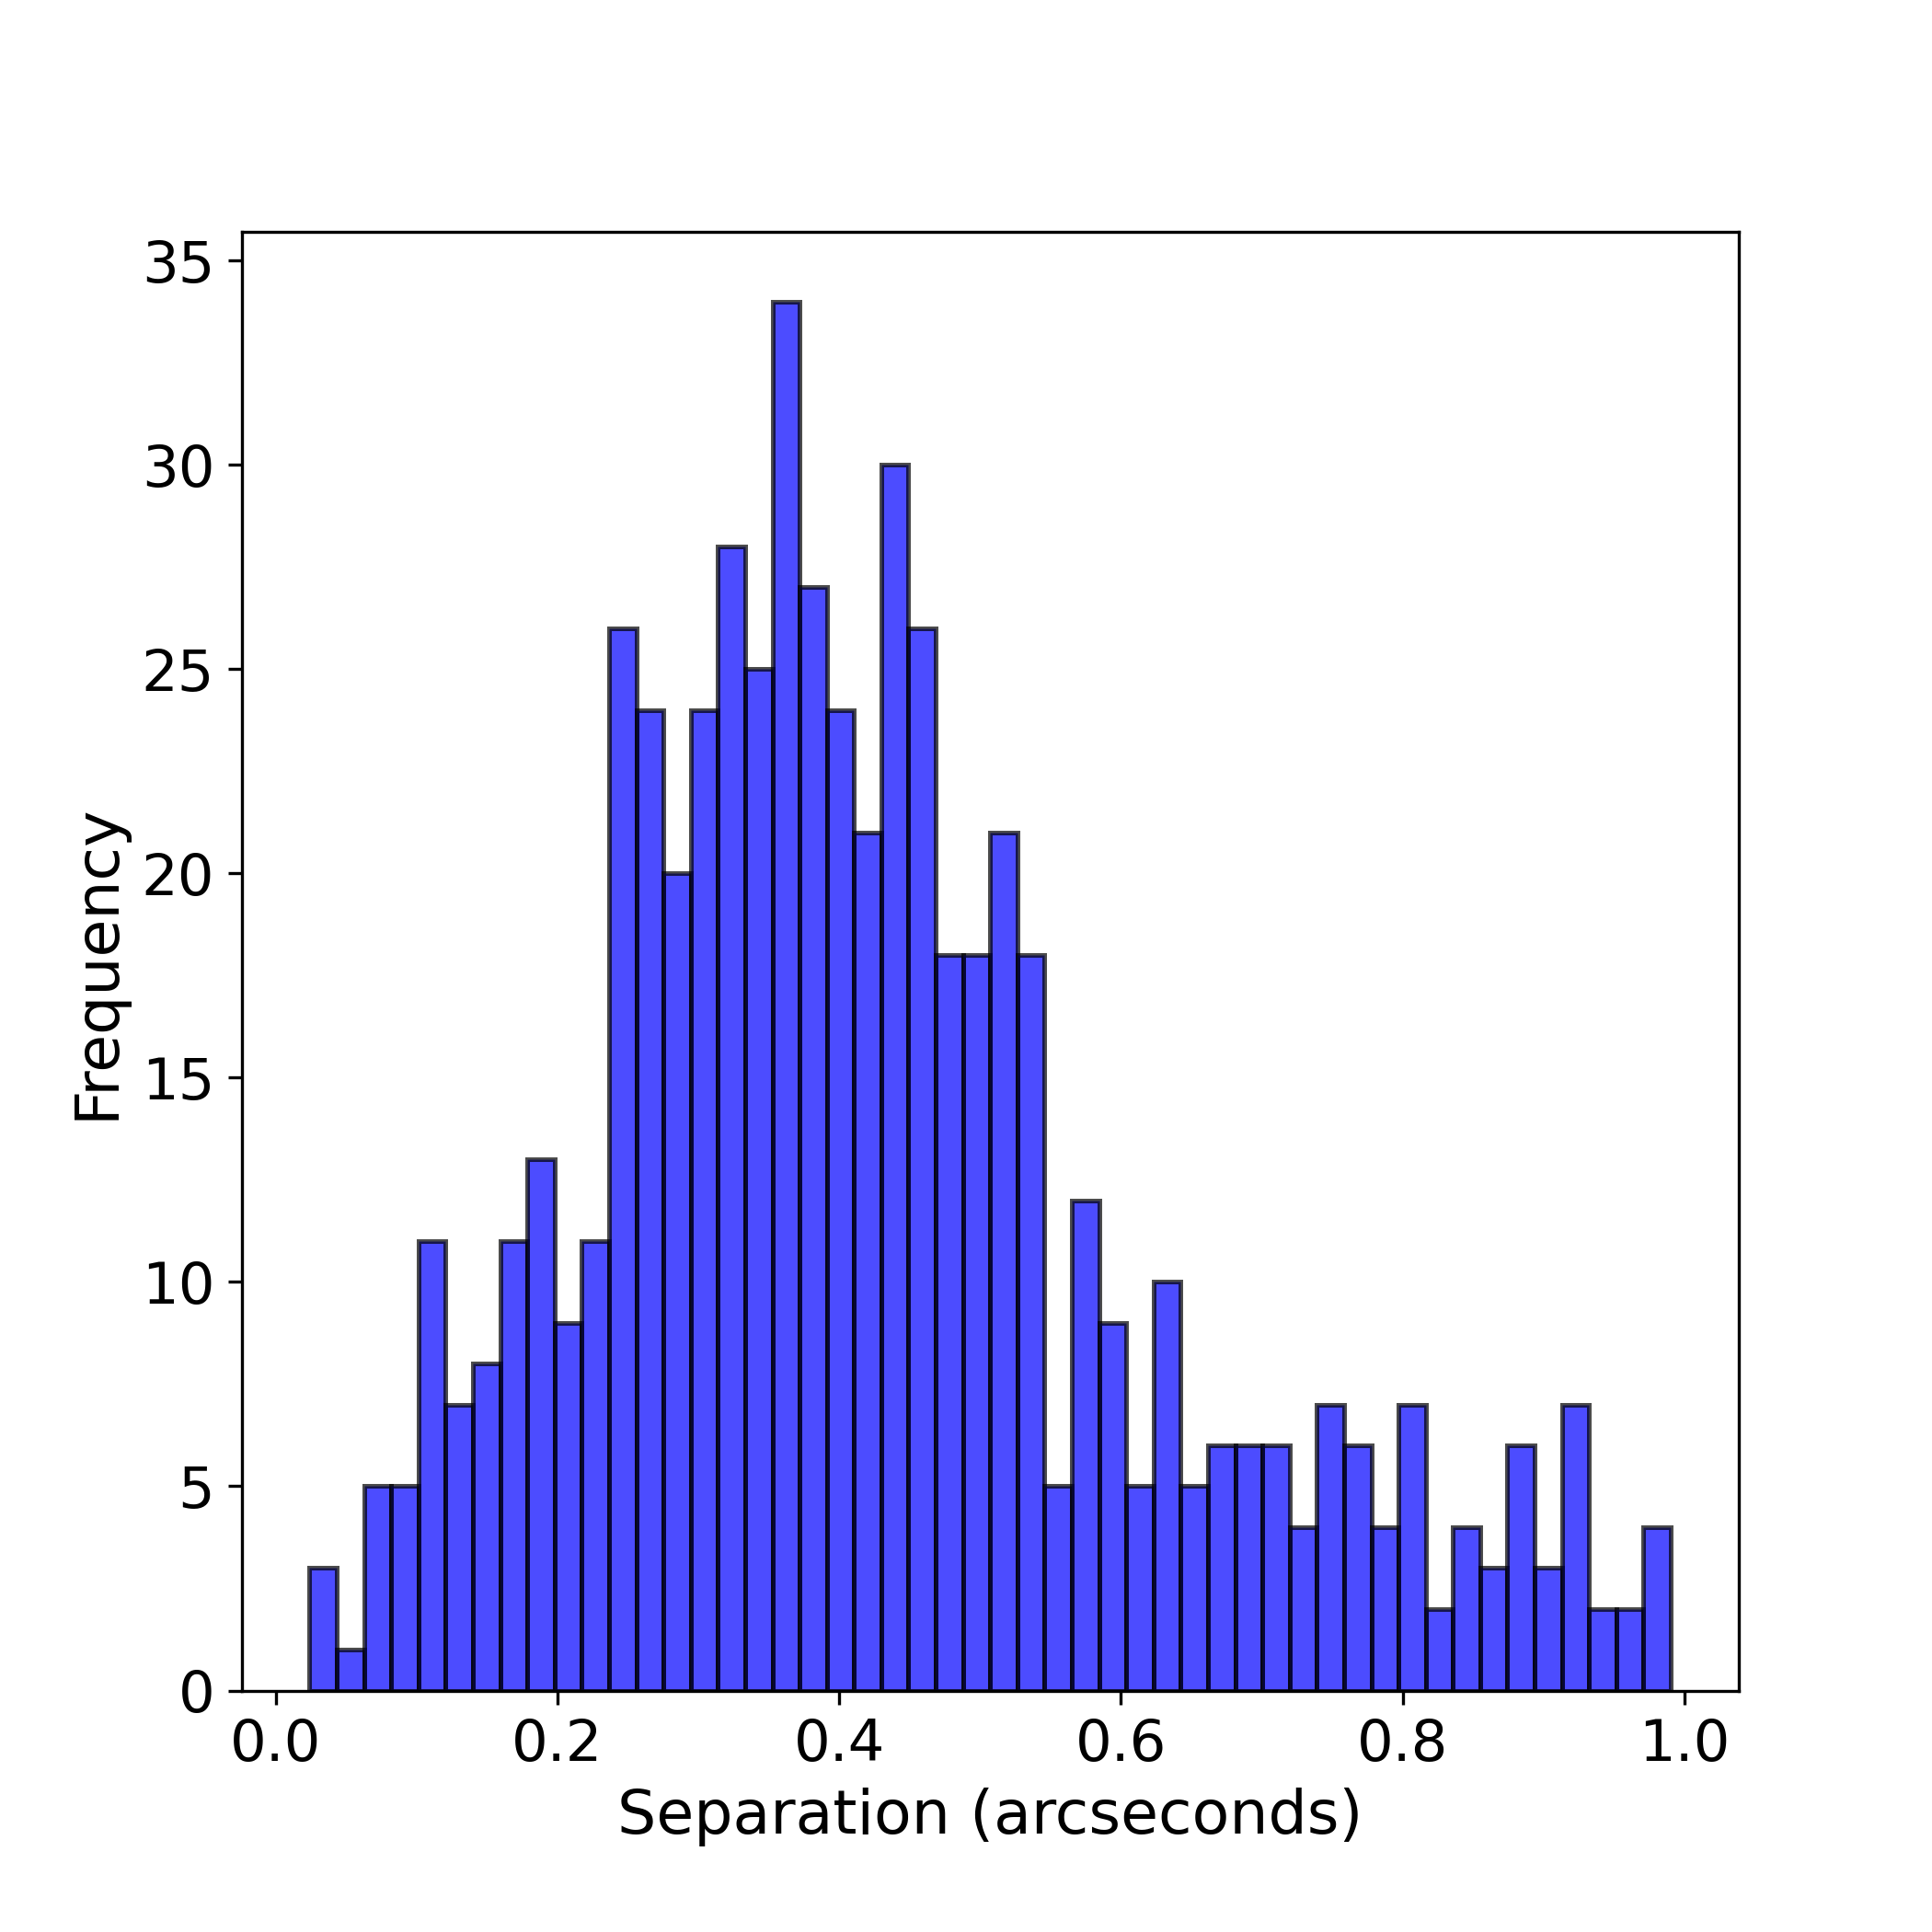
\includegraphics[width=0.49\textwidth]{plots/CDFS_4Ms_Xray_Sep.png}
  \caption{Distribution of arcsecond seperations for the CDFS 4Ms - ZFOURGE cross match.}
  \label{fig:ArcsecondSep}
\end{figure}
\section{Selection of AGN Candidates}
\subsection{Mid-Infrared Selections}
Dust-obscured AGN, which are challenging to observe in the optical spectrum, are relatively more accessible through infrared observations \cite{yutani_origin_2022}. In this project we use mid-infrared colour-colour selection techniques from Lacy \cite{lacy_obscured_2004, lacy_optical_2007}, Donley\cite{donley_spitzer_2007, donley_identifying_2012}, and Messias \cite{messias_new_2012, messias_dependency_2014} we aim to select AGN candidates in each of the legacy fields. For IR candidate selection we use a sample selection of galaxies that are selected via the use = 1 flag, This ensures that the source has good photometry, a reliable redshift, and hasn't been misidentified as a star \cite{straatman_fourstar_2016}. In addition to applying the use flag, we filter sources based on a flux-to-error ratio of 5, omitting sources with high flux error and subsequently reducing the error in the final selection.
\subsection{Lacy Wedge Selection}
The Lacy Wedge uses Spitzer colours from SDSS quasars to empirically define a colour selection that would select MIR SEDs that correspond to AGN \cite{lacy_obscured_2004}. To perform this selection, the selection uses IRAC fluxes at wavelengths of $3.6\mu m$, $4.5\mu m$, $5.8\mu m$, and $8.0\mu m$. Performing the colour-colour selection the sources were plotted with a x-axis colour of $log(f_{5.8}/f_{3.6})$ and a y-axis colour of $log(f_{8.0}/f_{4.5})$ and the colour selection criteria were applied to each field. The lacy selection criteria are given by
\begin{align*}
    \begin{split}
       \log_{10}\left(f_{5.8}/f_{3.6}\right)&>-0.1\\
       \log_{10}\left(f_{8.0}/f_{4.5}\right)&>-0.2\\
       \log_{10}\left(f_{8.0}/f_{4.5}\right)&<0.8\times\log_{10}\left(f_{5.8}/f_{3.6}\right)+0.5
    \end{split}
\end{align*}
\subsection{Donley Wedge Selection}
Donley builds upon previous work by selecting the best aspects from Lacy \cite{lacy_obscured_2004, lacy_optical_2007} and by Stern \cite{stern_midinfrared_2005} to develop a more robust selection technique \cite{donley_identifying_2012}. Similar to lacy, this selection uses IRAC fluxes at $3.6\mu m$, $4.5\mu m$, $5.8\mu m$, $8.0\mu m$, and the colour axes of $x = log(f_{5.8}/f_{3.6})$ and $y = log(f_{8.0}/f_{4.5})$. The Donley selection criteria were similarly applied to each field. The Donley selection criteria are given by
\begin{align*}
    x &\geq 0.08 \ \land y \geq 0.15 \ \land\\
    y &\geq (1.21 \times x) - 0.27 \ \land\\
    y &\leq (1.21 \times x) + 0.27 \ \land
\end{align*}
Where $\land$ is a logical OR operator. In addition to this, the fluxes must be well-constrained.
\begin{align*}
    \begin{split}
        &f_{4.5\, \mu\text{m}} > f_{3.6\, \mu\text{m}}\  \land\\ 
        \ &f_{5.8\, \mu\text{m}} > f_{4.5\, \mu\text{m}}\  \land\\
        \ &f_{8.0\, \mu\text{m}} > f_{5.8\, \mu\text{m}}
    \end{split}
\end{align*}
\subsection{Messias KI and KIM Selections}
The Messias KI and KIM selection are selection techniques that were developed based on the predictions of state-of-the-art galaxy and AGN templates \cite{messias_new_2012}. These techniques when used together are intended to cover the redshift range of $0 \leq z \leq 7$ \cite{messias_new_2012}. For this project, the KI technique is used over a redshift range of $0 \leq z \leq 1.8$ while the KIM technique is used over a redshift range of $1.8 \leq z \leq 3.2$. The Messias KI uses fluxes from the $K_s$ band, while also using IRAC fluxes at $4.5\mu m$ and $8.0\mu m$. The colour axes for the KI selection that were used were $x = [4.5] - [8.0]$ and $y = [K_s] - [4.5]$. For the KIM selection, this technique used the $24\mu m$ flux from the MIPS instrument along with the IRAC fluxes at $4.5\mu m$ and $8.0\mu m$. The colour axes for the KIM selection were $x = [4.5] - [8.0]$ and $y = [8.0] - [24]$. These techniques required that the fluxes be converted and plotted in the AB magnitude system used in the ZFOURGE paper \cite{straatman_fourstar_2016} using $\text{AB}_f =25-2.5\log_{10} \left( f \right)$ the fluxes were transformed and plotted in the colour-space for each respective field. The selection criteria that was used for KI and KIM is shown below
\begin{align*}
    \begin{split}
        z&<1.8\begin{cases}K_{s}-[4.5]>0&\\ [4.5]-[8.0]>0&\end{cases} \\
        z&>1.8\begin{cases}[8.0]-[24]>-2.9\times ([4.5]-[8.0])+2.8&\\ [8.0]-[24]>0.5&\end{cases}
    \end{split}
\end{align*}
\subsection{Szokoly X-Ray Selection}
The Szokoly X-ray selection techniques were used as they allow a simple and relatively reliable approach to selecting AGN based on the x-ray luminosity and hardness ratio of the source \cite{szokoly_chandra_2004}. This technique can select bright x-rays sources that may have been obscured by dust by examining the hardness ratio (HR) of a source. As the CDFS 4Ms Survey was crossmatched into ZFOURGE the x-ray selection was performed only in the CDFS field. The Szokoly x-ray selection technique is shown below
\begin{align*}
    L_x \geq \ 10^{41}\ erg\ s^{-1}\ \text{and}\ \text{HR} > -0.2 \\
    L_x \geq \ 10^{42}\ erg\ s^{-1}\ \text{and}\  \text{HR} \leq -0.2
\end{align*}
\subsection{Truth Sample, Completeness and Reliability}
As selection criteria can be influenced by contamination and incompleteness of data it is important to quantify these selections with a metric for the completeness and reliability of the sample. To determine the reliability and completeness the selected AGN must be compared against a truth sample of AGN. The truth sample is derived from the python Code Investigating Galaxy Emission (CIGALE) \cite{boquien_cigale_2019, yang_x-cigale_2020} which uses statistical models to generate and analyze SED data for galaxies. In this project, the selected AGN candidates are fed into CIGALE which outputs information about the source's AGN and dust luminosity contributions. If the luminosity contribution is $>50\%$ of the total luminosity, the source is marked as a known AGN. A selection is a positive diagnostic if it has both been marked by the selection diagnostic and as a known AGN. The completeness is defined as the fraction of positive diagnostics to known AGN, while the reliability is defined as the fraction of positive diagnostics to selected AGN. 
\begin{align*}
    \begin{split}
        \text{Completeness} &= N_{\text{AGN, SEL} }/N_{\text{AGN}}\\
        \text{Reliability} &= N_{\text{AGN, SEL} }/N_{\text{SEL}}
    \end{split}
\end{align*}
\section{Results}
\subsection{AGN Candidates}
This
\begin{table}[h]
\caption{\label{label}AGN Candidates selected using MIR and x-ray techniques.}
\begin{indented}
\item[]\begin{tabular}{@{}llllll}
\br
&Lacy&Donley&Messias&X-ray&Unique\\
\mr
CDFS & 874 & 123 & 45 & 137 & 1014 \\
COSMOS & 241 & 51 & 50 & n/a & 253 \\
UDS & 375 & 78 & 54 & n/a & 382 \\
Total & 1490 & 252 & 149 & 137 & 1649 \\
\br
\end{tabular}
\end{indented}
\end{table}
\begin{figure}[h]
  \centering
  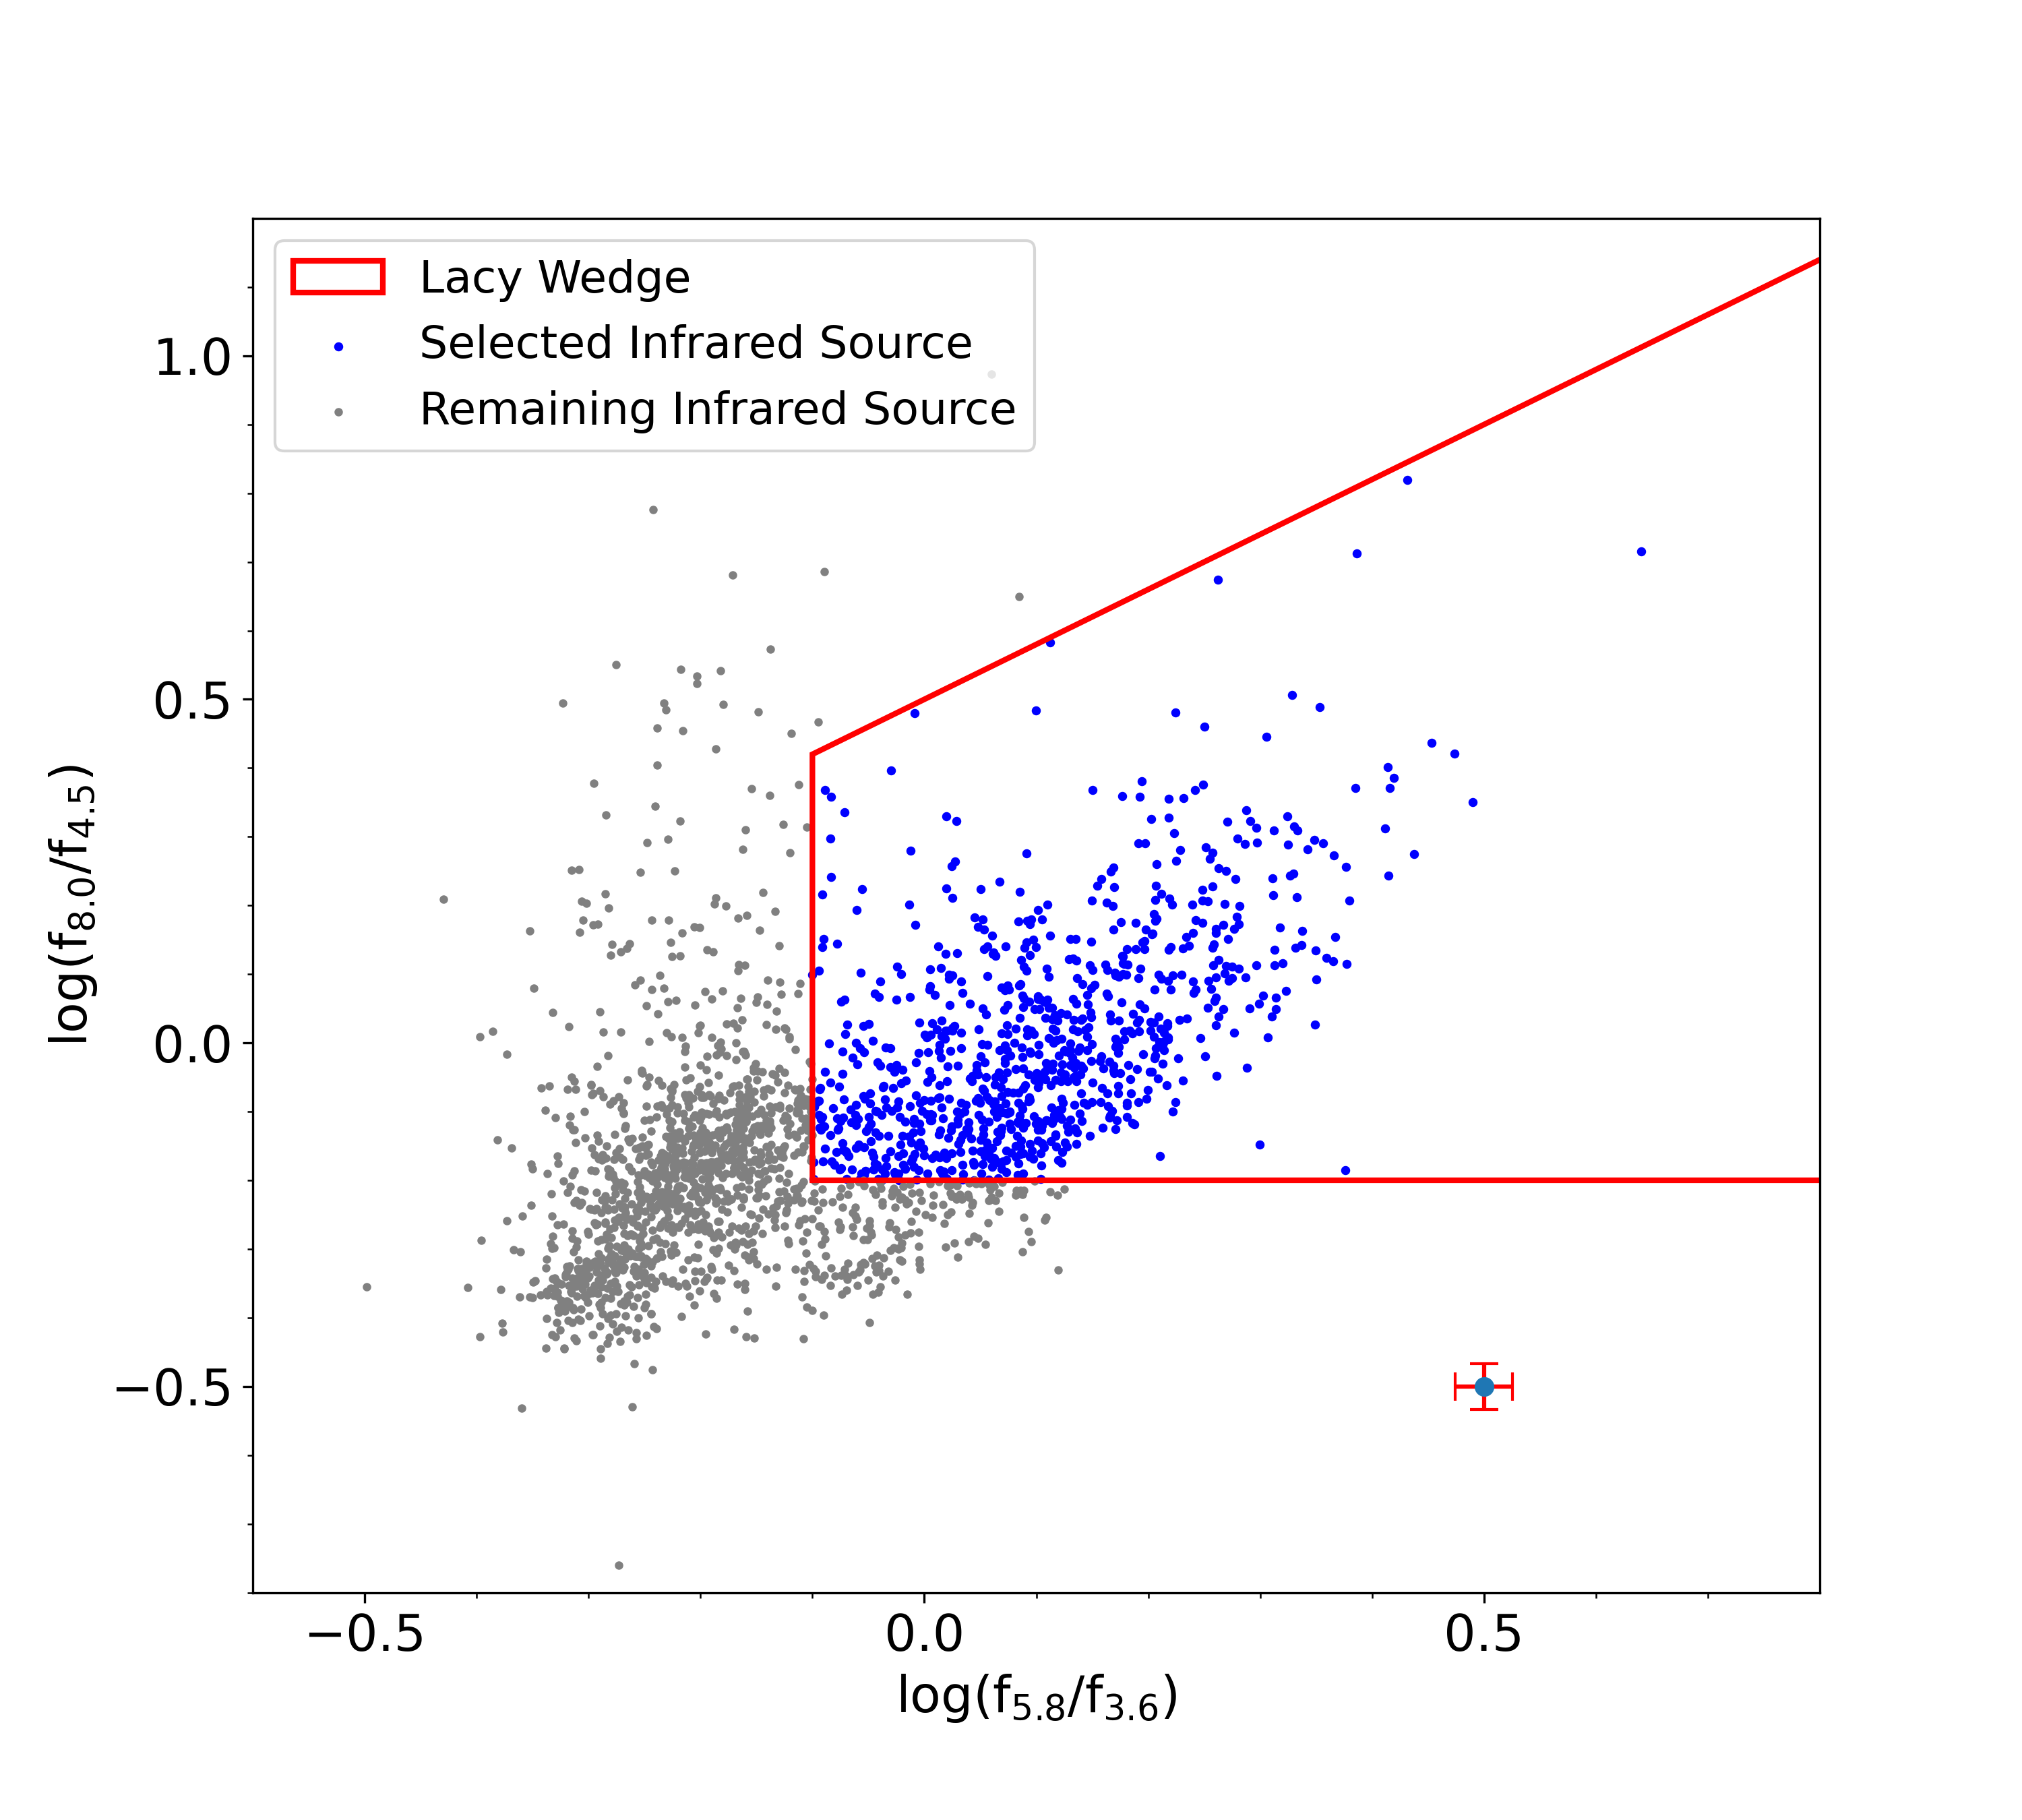
\includegraphics[width=0.49\textwidth]{plots/CDFSLacyWedge_error.png}
  \caption{The Lacy Wedge Selection for AGN candidates in the CDFS field. The average error is shown in the bottom right, propogated from flux}.
  \label{fig:LacyWedge}
\end{figure}
\begin{figure}[h]
  \centering
  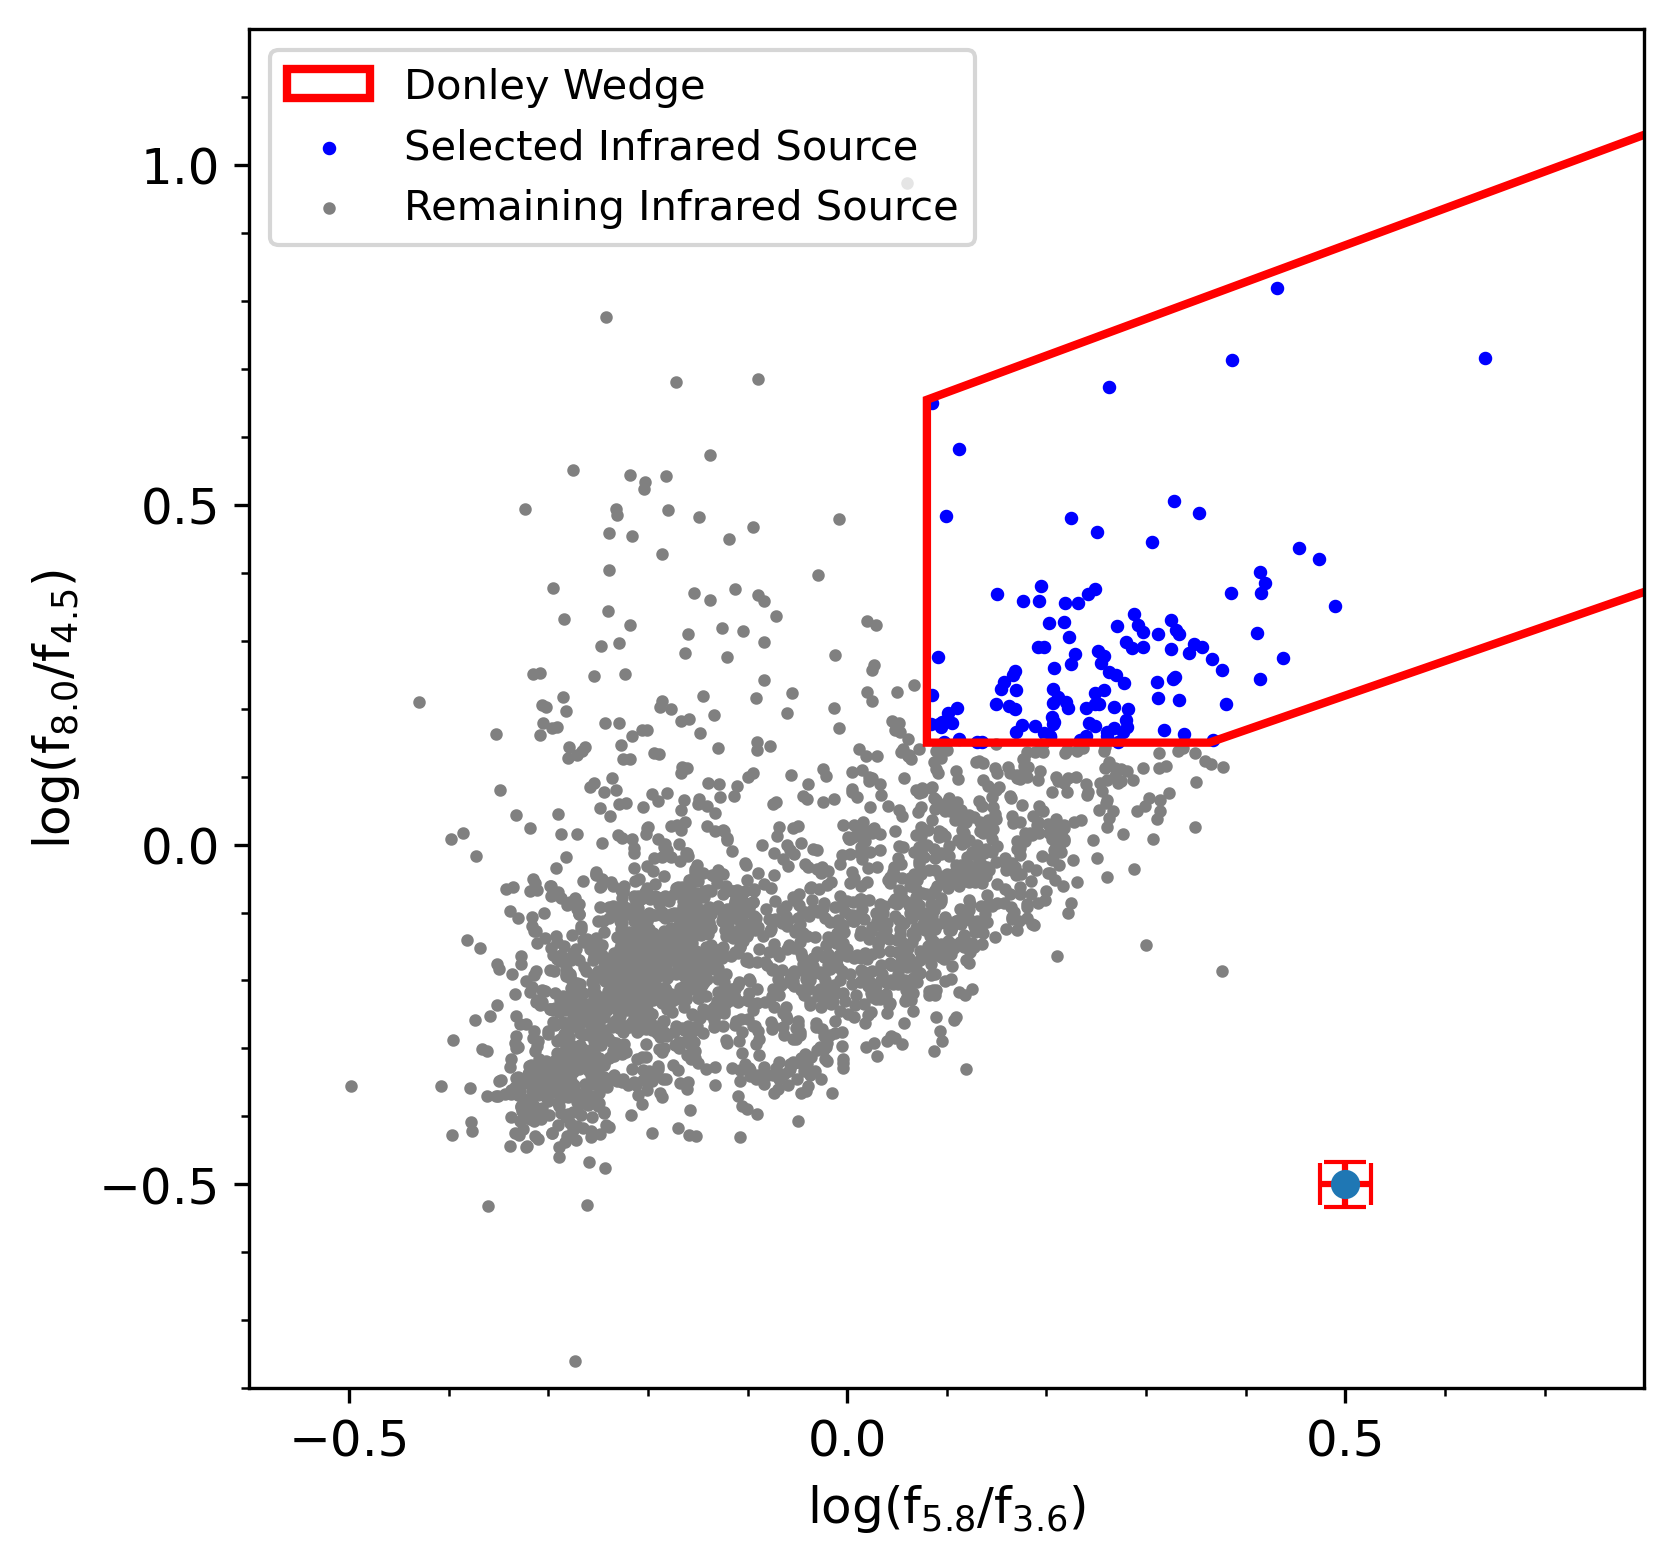
\includegraphics[width=0.49\textwidth]{plots/CDFSDonleyWedge_error.png}
  \caption{The Donley Wedge Selection for AGN candidates in the CDFS field. The average error is shown in the bottom right, propogated from flux.}
  \label{fig:DonleyWedge}
\end{figure}
\begin{figure}[h]
  \centering
  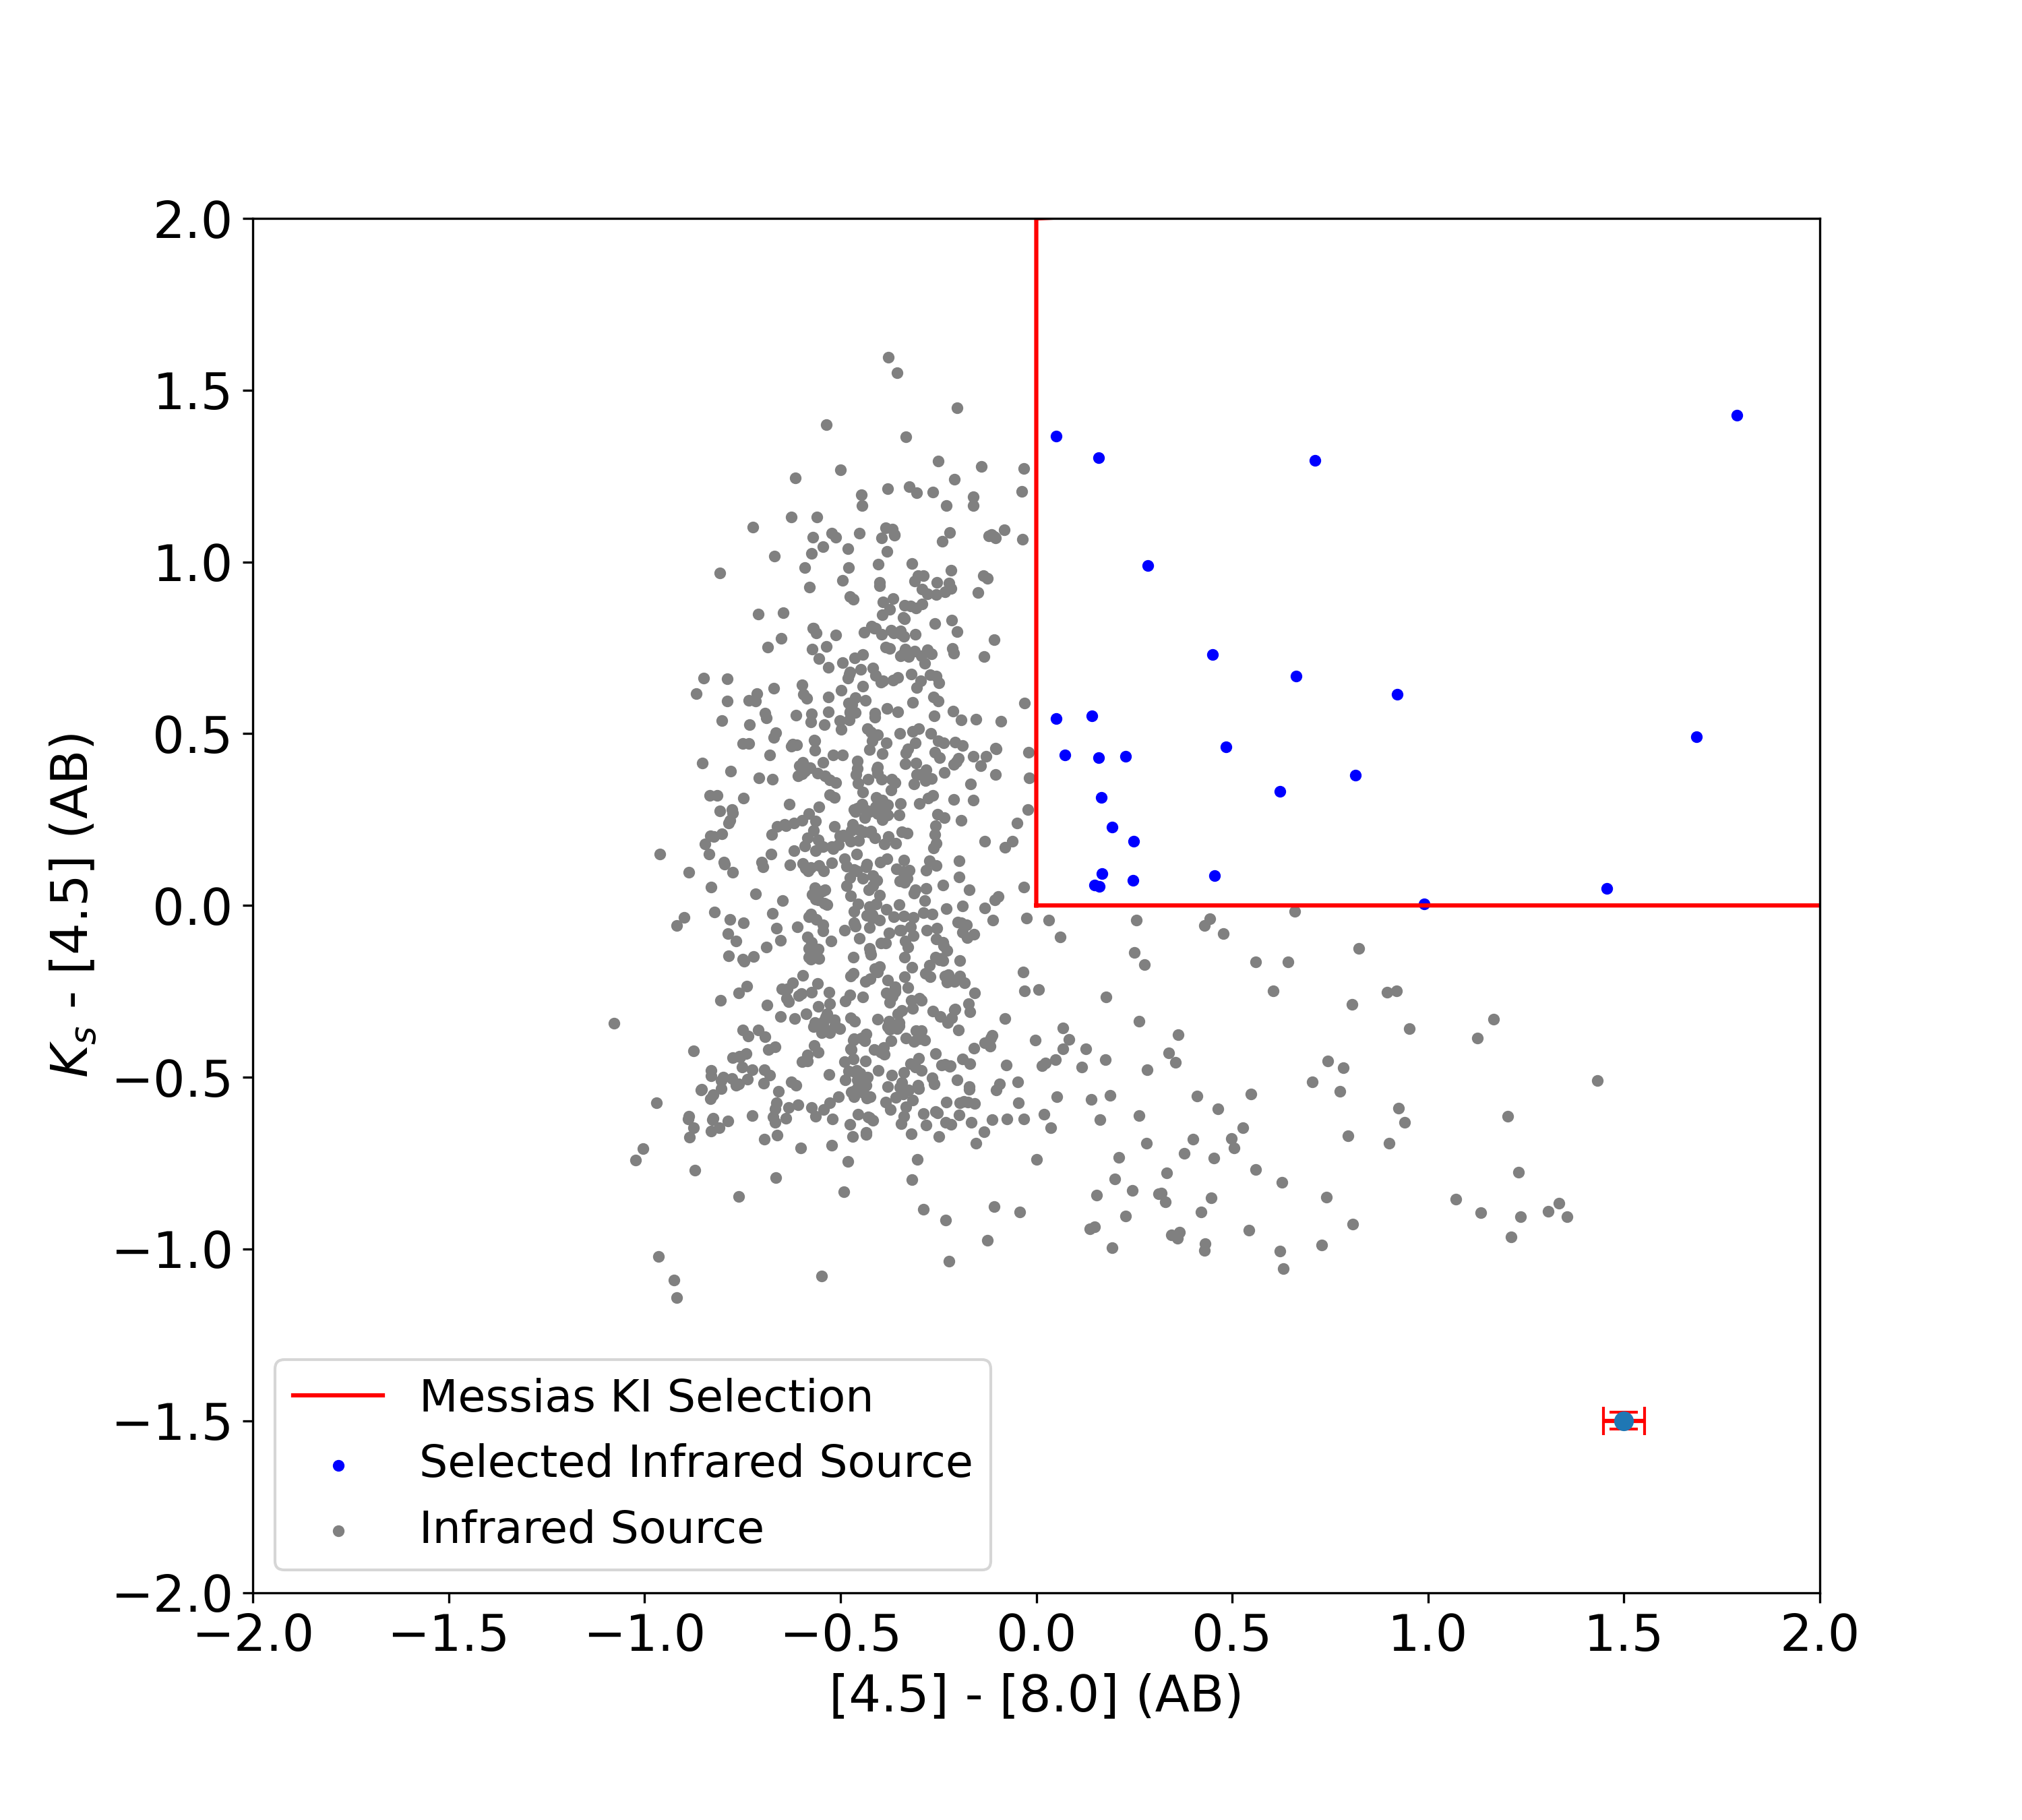
\includegraphics[width=0.49\textwidth]{plots/CDFSMessiasKISelection_error.png}
  \caption{The Messias KI Selection for AGN candidates in the CDFS field. This selection selects AGN with redshift $0.2 < z < 1.8$. The average error is shown in the bottom right, propagated from flux.}
  \label{fig:MessiasKI}
\end{figure}
\begin{figure}[h]
  \centering
  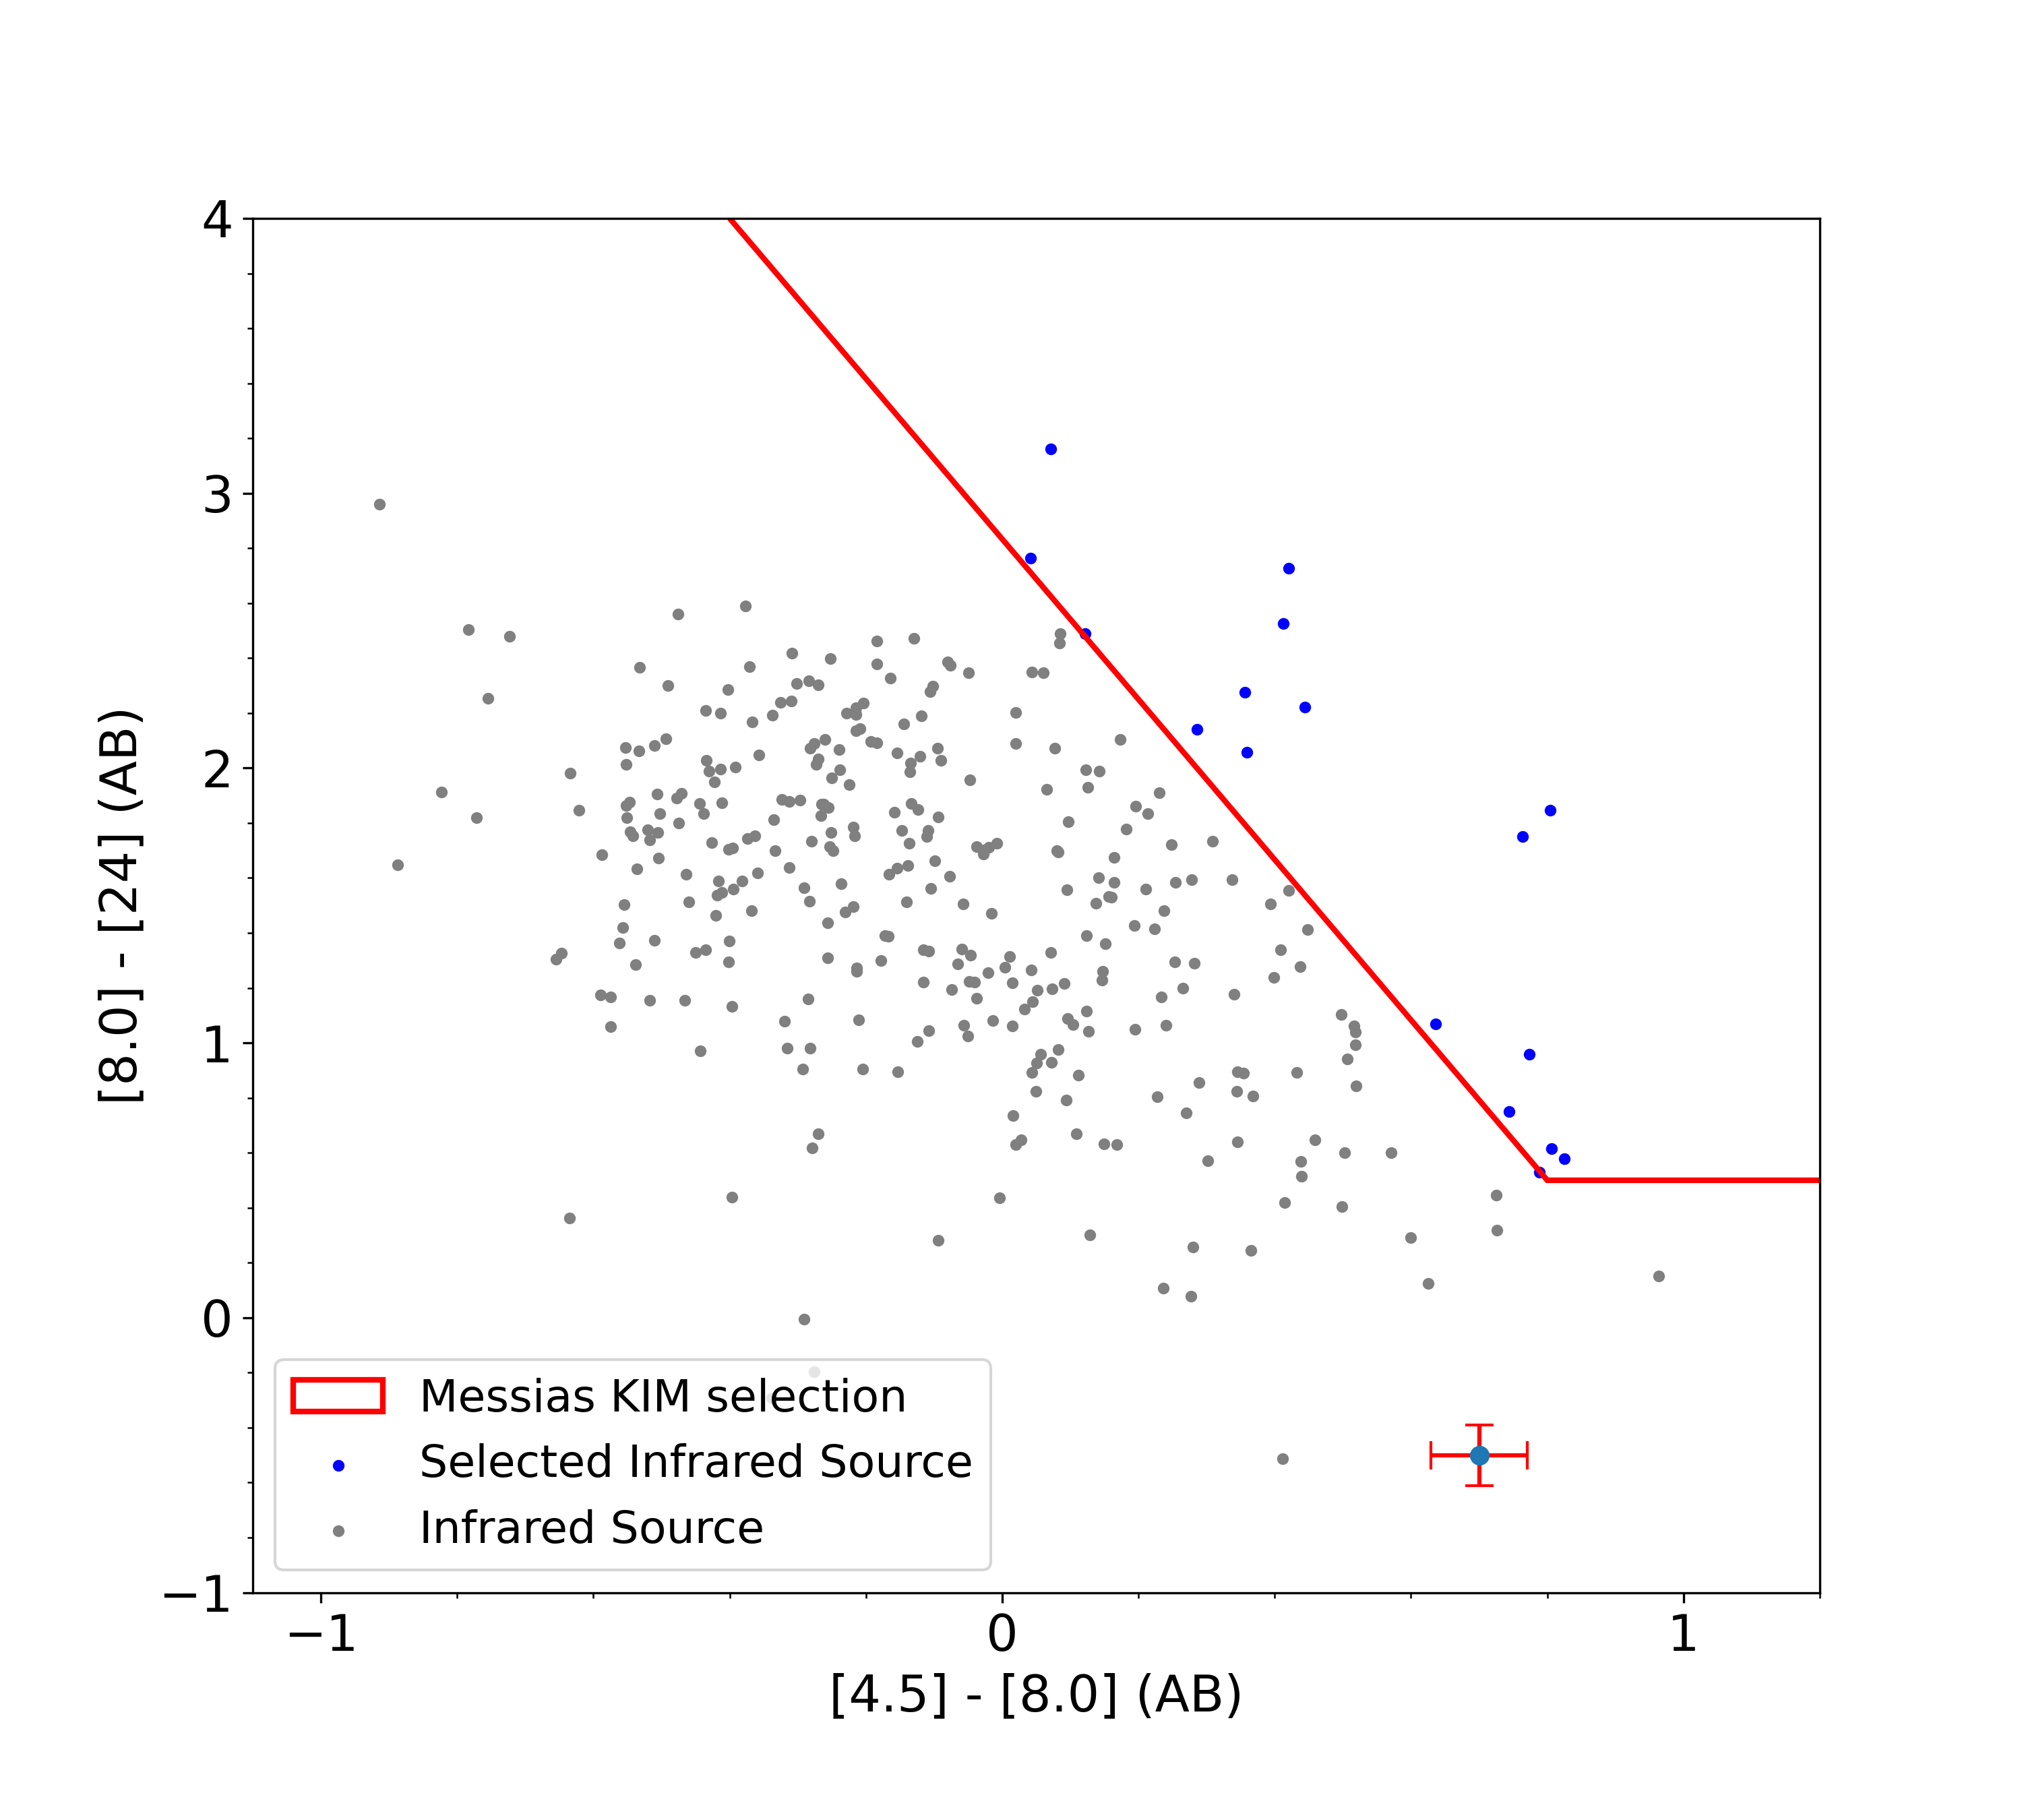
\includegraphics[width=0.49\textwidth]{plots/CDFSMessiasKIMSelection_error.png}
  \caption{The Messias KIM Selection for AGN candidates in the CDFS field. This selection selects AGN with redshift $1.8 < z < 3.2$. The average error is shown in the bottom right, propagated from flux.}
  \label{fig:Messias}
\end{figure}
\subsection{Completeness and Reliability of Selection}
\begin{figure}[h]
  \centering
  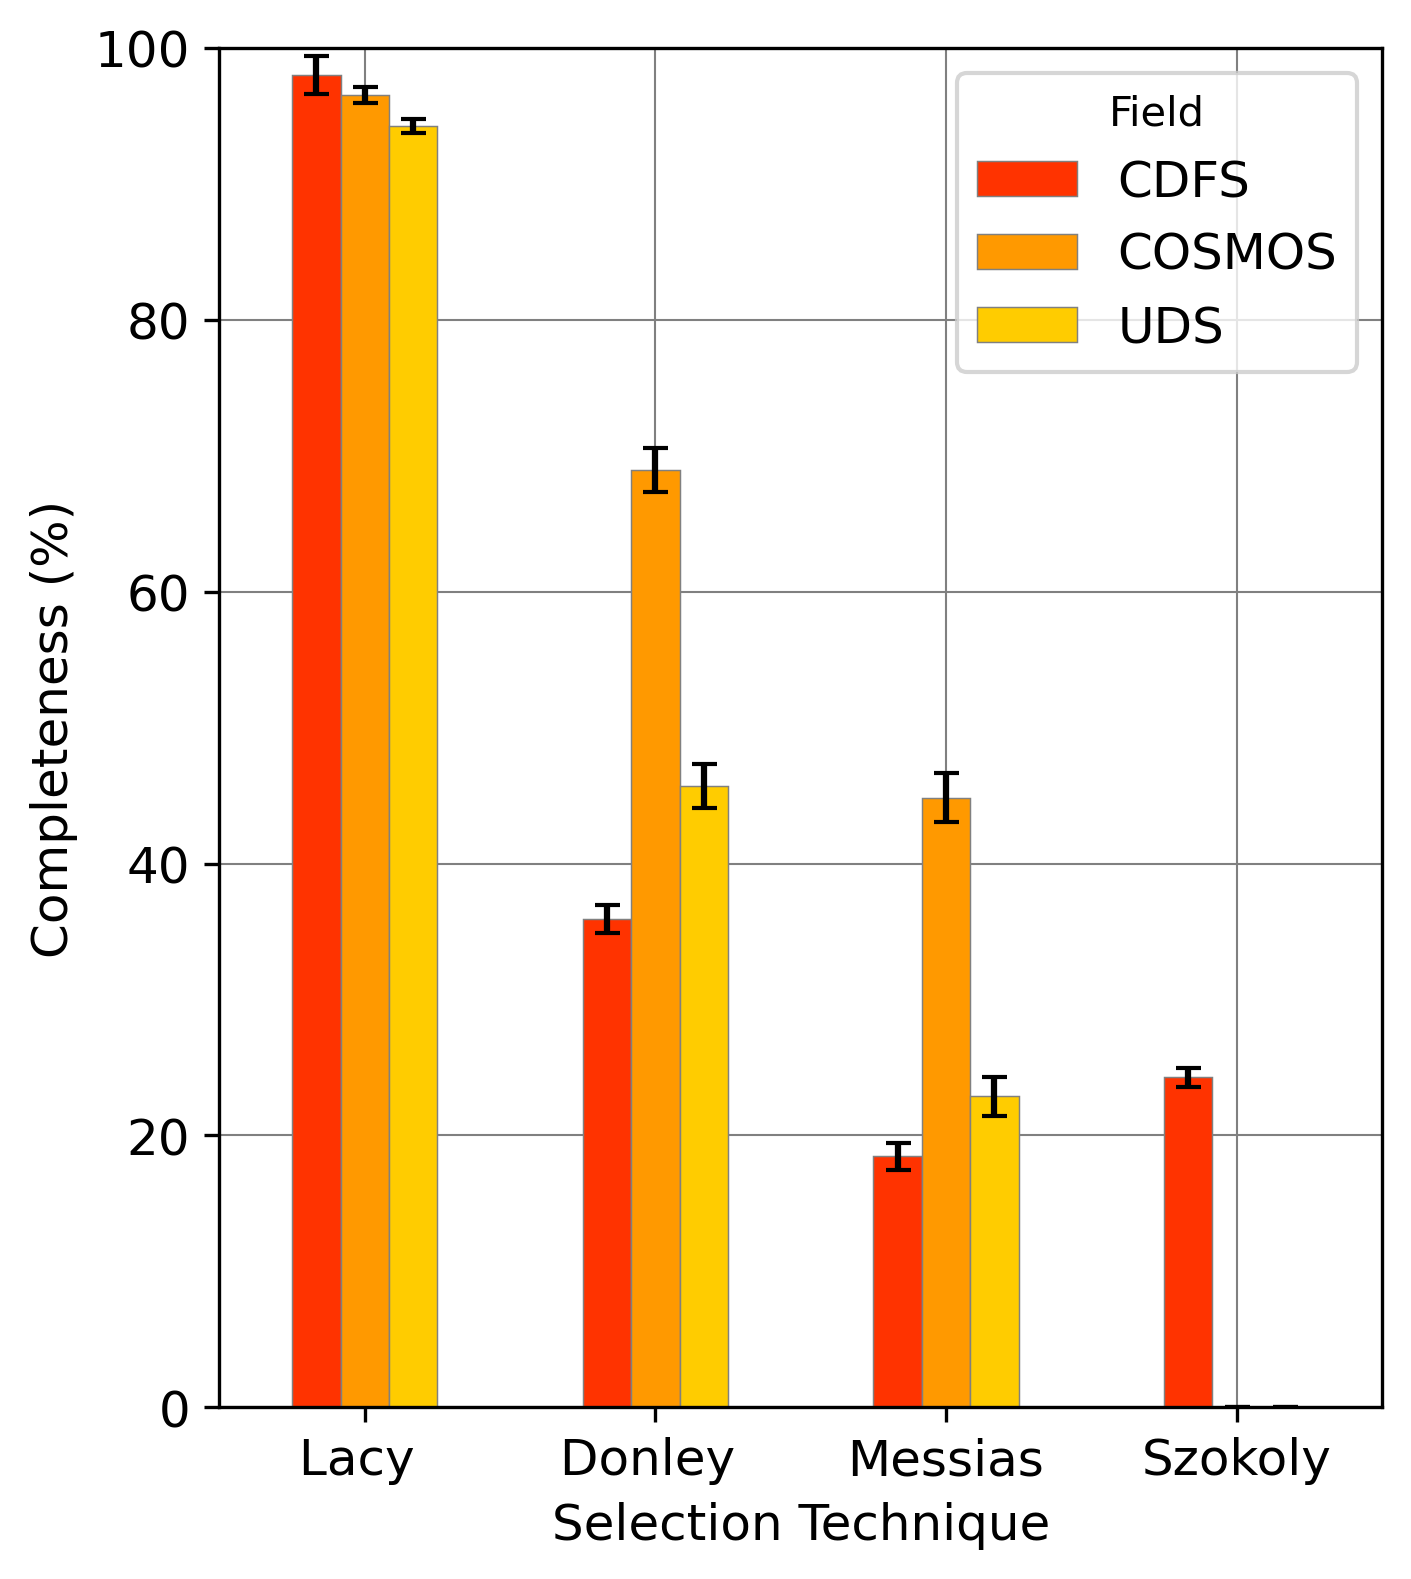
\includegraphics[width=0.40\textwidth]{plots/TechniqueCompleteness.png}
  \caption{The completeness for each technique in all fields}
  \label{fig:Completeness}
\end{figure}
\begin{figure}[h]
  \centering
  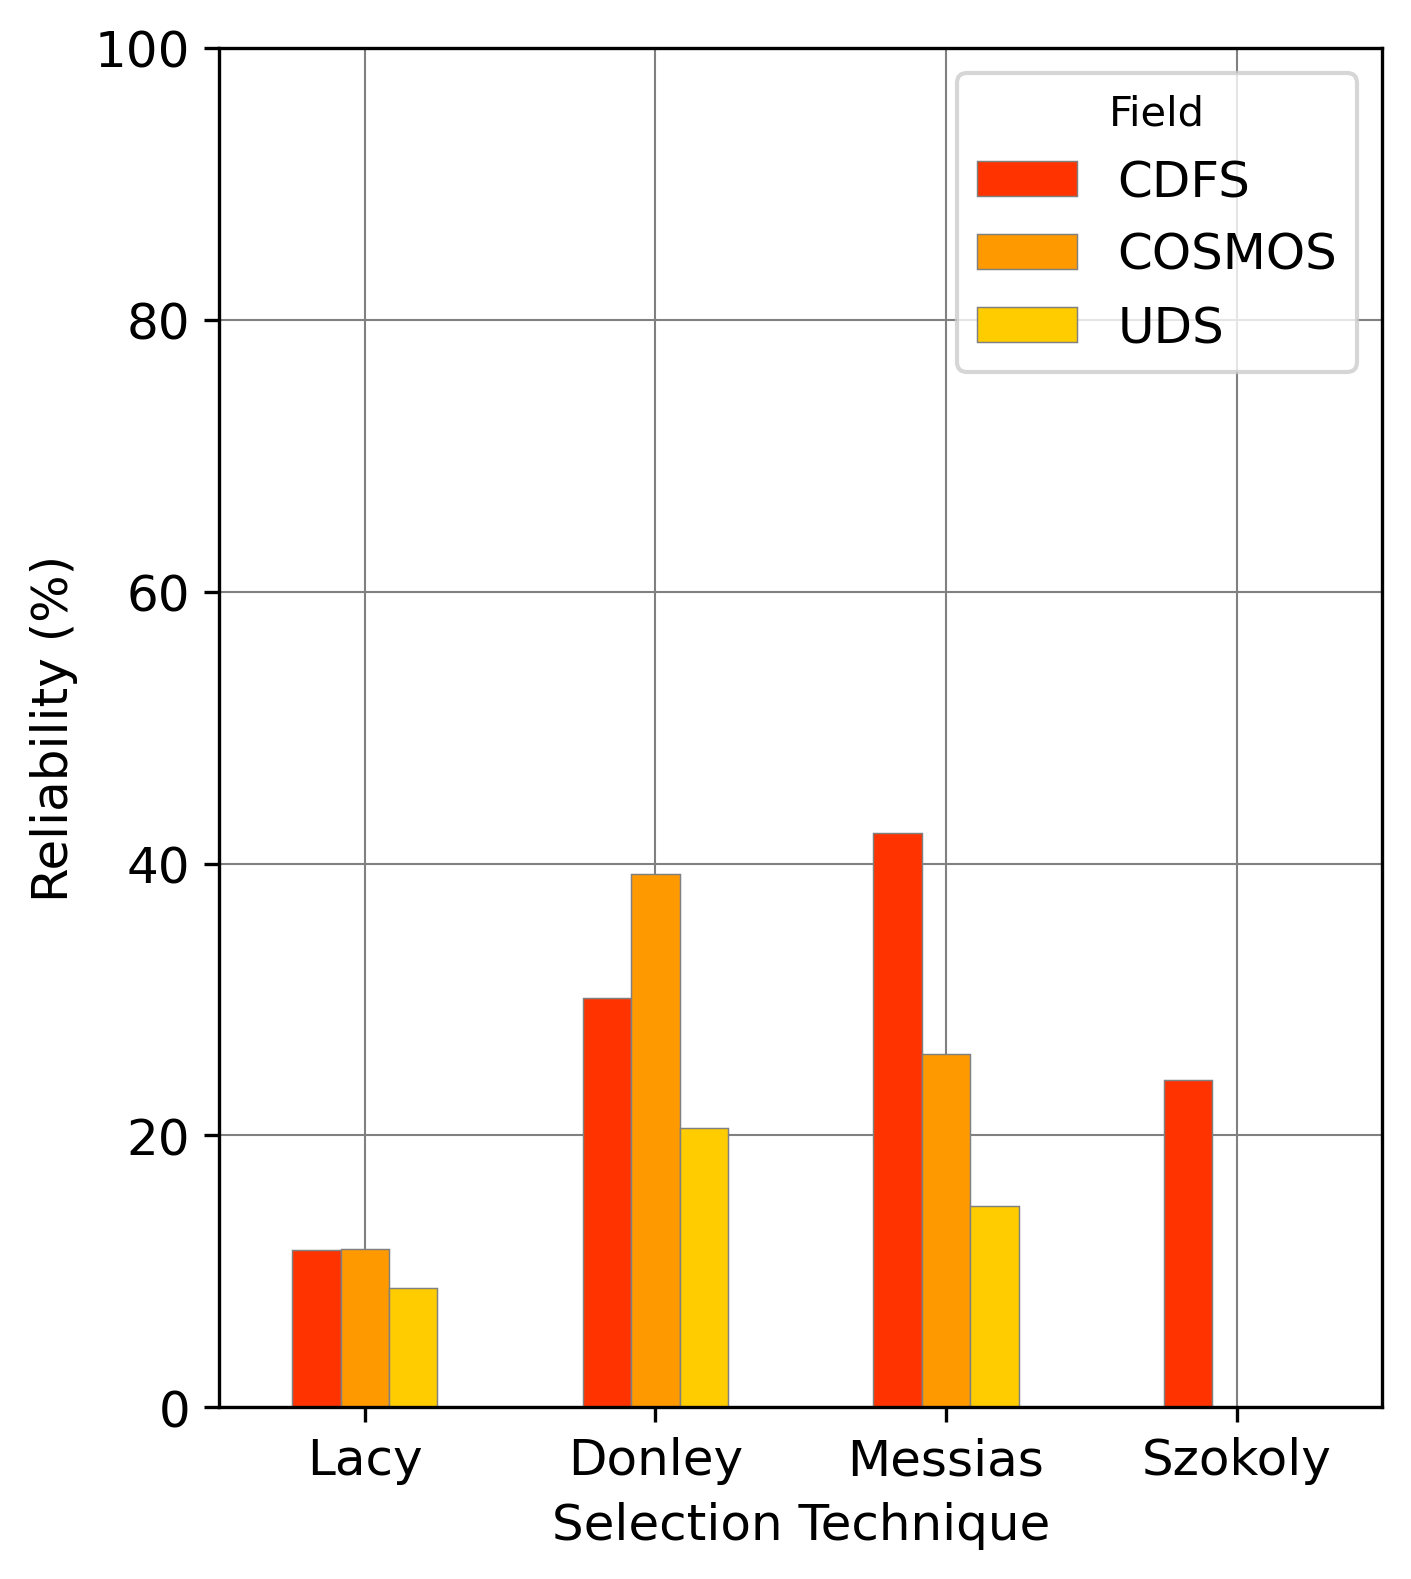
\includegraphics[width=0.40\textwidth]{plots/TechniqueReliability.png}
  \caption{The reliability for each technique in all fields}
  \label{fig:Completeness}
\end{figure}

\newpage
\section{Discussion}
\section{Conclusion}
\section{Acknowledgements}
\newpage
\section{References}
\bibliographystyle{vancouver}
\bibliography{report/references}
%\bibliography{references.bib} % references file!

%\bibliographystyle{vancouver} % referencing style


\end{document}